\chapter*{Approach}
\addcontentsline{toc}{chapter}{Approach}

The development of a streaming data processing pipeline is a complex undertaking that requires careful selection of technologies at each architectural layer. Dozens of tools and deployment options exist for implementing such pipelines, ranging from self-managed on-premises services to fully managed cloud-native SaaS solutions.

Most modern data pipelines are structured around three principal stages: extraction, transformation, and loading (ETL). This chapter examines the technologies employed at each of these stages, justifies the architectural choices made, and discusses the simulation of data generation and the visualization of processed results.

\section*{Research Objectives and Scope}

The objective of this work is the design, implementation, and deployment of a cloud-native streaming data processing pipeline that guarantees end-to-end latency of less than one minute between the stages of data generation and data visualization.

The data generation stage itself is outside the primary scope of this work. The principal focus is placed on the ingestion, processing, and storage of streaming data, as well as its visualization using appropriate analytical tools.

\section*{Pipeline Architecture}

The system is organized around two boundary components: a data generator — implemented in this work as a microservices simulator — and a visualization layer consisting of analytical dashboards.

As illustrated in Figure~\ref{fig:dataflow}, between these two boundary components lie the core elements of the pipeline: an event queue, a stream processing engine, and an analytical data warehouse. Each component fulfils a distinct role: the event queue provides reliable buffering and decoupling of producers from consumers; the stream processing engine performs continuous transformation and aggregation of incoming events; the storage layer persists aggregated results for downstream querying; and the visualization layer presents those results to stakeholders in an interpretable form.

\begin{figure}[H]
    \centering
    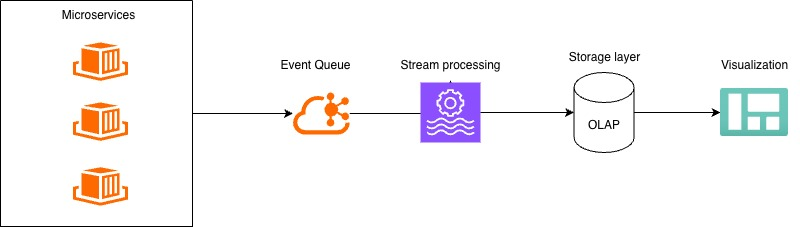
\includegraphics[width=1\textwidth]{Figures/Data flow.jpg}
    \caption{Architecture of the streaming data processing pipeline, illustrating the main system components and the direction of data flow.}
    \label{fig:dataflow}
\end{figure}

\subsection*{Data Production}

In production environments, analytics data originates from a wide variety of sources — including replication of operational databases, in-application event streaming, and third-party integrations. Since the primary focus of this work is on pipeline architecture rather than business logic, event stream generation is simulated using a lightweight service implemented in Python with the FastAPI framework.

FastAPI was selected for this purpose due to its minimal overhead and its straightforward interface for defining HTTP endpoints. To facilitate controlled testing and reproducible experimentation, the simulator exposes two configurable parameters: the event generation rate and the total number of events to be produced. Once generated, events are dispatched to the messaging system, which is responsible for their reliable delivery and subsequent ingestion by downstream pipeline components.

\subsection*{Stream Processing Engine}

The selection of an appropriate stream processing engine is a critical architectural decision, as it is the primary factor determining pipeline latency, maintainability, and capacity for future extension. Three candidate technologies were evaluated: Apache Spark Streaming, Apache Flink and Apache Storm.

Apache Spark Streaming is one of the earliest frameworks for large-scale stream processing. However, its micro-batch execution model introduces inherent latency overhead, as data is processed in discrete intervals rather than continuously \cite{joy2024scalable}. Given that minimising end-to-end latency between event generation and dashboard visualisation is a core requirement of this work, this execution model presents an unacceptable architectural risk.

Apache Storm is similarly one of the earliest distributed stream processing frameworks, offering record-at-a-time processing with low latency. Nevertheless, it has been largely superseded by more modern alternatives that provide superior throughput, more accessible APIs, and stronger processing guarantees \cite{joy2024scalable}.

Apache Storm is similarly one of the earliest distributed stream processing frameworks, offering record-at-a-time processing with low latency. Nevertheless, it has been largely superseded by more modern alternatives that provide superior throughput, more accessible APIs, and stronger processing guarantees \cite{joy2024scalable}.

Apache Flink was therefore selected as the stream processing engine for this pipeline. Unlike Spark Streaming, Flink operates on a true event-at-a-time execution model, processing each record as it arrives rather than accumulating micro-batches, which is essential for achieving sub-minute latency. Empirical evaluation reported by Joy \cite{joy2024scalable} demonstrates that Flink achieves an average latency of approximately 100\,ms at a throughput of 100,000 events per second — a performance profile that satisfies the requirements of this project. Beyond raw performance, Flink provides a rich set of APIs with native support for event-time semantics, watermarking, stateful operators, and windowed aggregations, enabling correct processing of out-of-order events \cite{carbone2020beyond}. Finally, Flink is a mature, well-documented open-source project backed by an active community, with production deployments at significant scale demonstrating its reliability \cite{carbone2020beyond} — factors that further distinguish it from less established alternatives.

\subsection*{Data Storage}

The choice of a storage layer is equally as critical as the selection of a stream processing engine. For the purposes of this work, the storage solution must support not only efficient data persistence, but also low-latency reads and, where necessary, on-the-fly aggregation of query results. Three candidate technologies were evaluated: ClickHouse and DuckDB for the local deployment environment, and Amazon Redshift for the cloud deployment environment.

DuckDB is an analytical database designed for single-node deployments. It operates without a dedicated server process, making it easy to set up and integrate into existing applications. DuckDB employs a columnar storage format with vectorised query execution, delivering competitive analytical performance for datasets that fit within the capacity of a single machine \cite{duckdb}. However, its single-node architecture precludes horizontal scaling, and its support for concurrent writes from multiple producers is limited. For these reasons, DuckDB does not provide the ingestion throughput or scalability required by this pipeline and was therefore excluded from further consideration.

Amazon Redshift is a fully managed, cloud-native data warehouse provided by AWS, built on a massively parallel processing (MPP) architecture. It offers deep integration with the broader AWS ecosystem — including native connectors for S3, Kinesis, and Glue — and supports standard SQL with PostgreSQL-compatible syntax \cite{kumar2025evolution}. These characteristics make it a natural fit for pipelines deployed exclusively on AWS. However, Redshift is optimised for large-scale batch analytical workloads rather than continuous, low-latency ingestion. Data written to Redshift is not immediately available for querying, as the platform requires a commit and refresh cycle that introduces latency between the moment of ingestion and query availability. Additionally, as a proprietary managed service, Redshift introduces vendor lock-in and cannot be reproduced in a local deployment environment — a requirement of this work.

ClickHouse is an open-source, column-oriented database management system designed specifically for high-throughput analytical workloads. Its MergeTree storage engine provides efficient columnar compression and supports high-velocity concurrent writes, making it well-suited for continuously persisting aggregated results produced by the stream processing engine. Empirical benchmarks indicate that ClickHouse consistently outperforms alternative OLAP engines on complex aggregation queries, achieving query latencies in the millisecond range even at significant data volumes \cite{clickbench}. Unlike Redshift, ClickHouse is deployment-agnostic and can be configured identically across both local Docker-based environments and AWS EC2 instances. For these reasons, ClickHouse was selected as the storage layer for this pipeline.

\subsection*{Data Visualization}

The visualization layer is responsible for presenting aggregated results stored in the analytical database to end users in an interpretable and timely manner. Three candidate technologies were evaluated: Apache Superset, Grafana, and Amazon QuickSight.

Apache Superset is an open-source business intelligence platform originally developed at Airbnb. It provides a broad range of visualization types and a flexible SQL-based query interface. Superset supports ClickHouse natively through a dedicated database connector and can be deployed consistently across both local and cloud environments. However, its minimum auto-refresh interval is approximately 10 seconds, which, while technically sufficient for the latency requirement of this work, represents a limitation for use cases demanding more frequent updates.

Amazon QuickSight is a fully managed, cloud-native business intelligence service provided by AWS. It offers seamless integration with the AWS ecosystem, including native connectors for Redshift, S3, and Athena. However, QuickSight's integration with ClickHouse requires a custom JDBC connector, adding considerable configuration complexity. More critically, as a proprietary AWS-managed service, QuickSight cannot be deployed in a local environment. For these reasons, QuickSight was excluded from further consideration.

Grafana is an open-source analytics and monitoring platform widely adopted for real-time observability workloads. It provides an official ClickHouse plugin maintained by the ClickHouse team. Grafana supports dashboard auto-refresh intervals as low as one second, providing the responsiveness required by this pipeline. This aligns with the performance optimization strategies outlined by Lukianets and Sulema \cite{lukianets2023visualization}, who identify caching and efficient data delivery as critical factors in sustaining real-time visualization performance under high data velocity. Furthermore, Grafana can be deployed identically in both local Docker-based environments and on AWS. For these reasons, Grafana was selected as the visualization layer for this pipeline.

\section*{Deployment Environments}

\subsection*{Local Environment}

\subsection*{AWS Cloud Environment}

\section*{Measurement Methodology}

\subsection*{Latency Definition}

\section*{Limitations}

\section*{Summary}
